%\subsection{Définition des  n\oe uds}
\SbSSCT{Définition des  n\oe uds}{Creation of nodes}
\tikzset{blue}

\begin{tabular}{|c | c | c | c |} \hline
\multicolumn{4}{|c|}{  \BS{draw} (1,1) node[\RDD{fill}=red!20] \AC{};   }\\ 
\hline 
\tikz \draw (0,0) grid (2,2) (1,1) node[fill=red!20] {};
&
\tikz \draw (0,0) grid (2,2) (1,1) node[fill=red!20,draw] {}; 
&
\tikz \draw (0,0) grid (2,2) (1,1) node[circle,fill=red!20] {};
&
\tikz \draw (0,0) grid (2,2) (1,1) node[circle,fill=red!20,draw] {};
\\  \hline
\dft
&
node[\RDD{draw}] 
&
 node[\RDD{circle}]  
&
 node[\RDD{circle},\RDD{draw}]
 \\  \hline
\end{tabular}
\bigskip

\begin{tabular}{|c | c | c | c |} \hline
\multicolumn{4}{|c|}{ \BSS{node} \RDD{at} (1,1) [fill=red!20] \AC{};   }\\ 
\hline 
 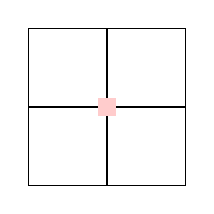
\begin{tikzpicture}
\draw (0,0) grid (2,2) ; 
\node at (1,1) [fill=red!20] {};
 \end{tikzpicture}
&
 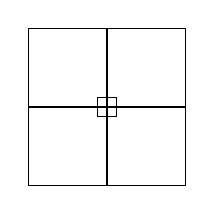
\begin{tikzpicture}
\draw (0,0) grid (2,2) ; 
\node at (1,1) [draw] {};
 \end{tikzpicture}
&
 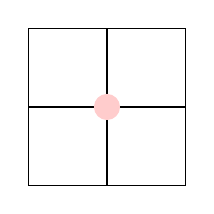
\begin{tikzpicture}
\draw (0,0) grid (2,2) ; 
\node at (1,1) [fill=red!20,circle] {};
 \end{tikzpicture}
&
 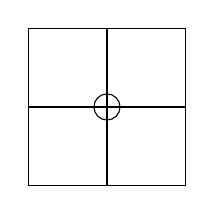
\begin{tikzpicture}
\draw (0,0) grid (2,2) ; 
\node at (1,1) [circle,draw] {};
 \end{tikzpicture}
\\  \hline
[fill=red!20]
&
[\RDD{draw}] 
&
[\RDD{circle},fill=red!20]
 &
[\RDD{circle},draw] 
 \\  \hline
\end{tabular}
\bigskip

\TFRGB{Autres types de n\oe uds voir page}{Other type of nodes see page} \pageref{noeudboite}



%-------------------------------------------------------------------------------
%\subsection{Liaisons}
\SbSSCT{Liaisons}{Links}
\label{liaisons}

\begin{tabular}{|c|c|c|} \hline  
\begin{tikzpicture}[blue]
\node[draw] (A) at (0,0) {A};
\node[draw] (B) at (1.5,1.5) {B};
\draw (A) -- (B);
\end{tikzpicture}
&  
\begin{tikzpicture}[blue]
\node[draw] (A) at (0,0) {A};
\node[draw] (B) at (1.5,1.5) {B};
\draw (A) |- (B);
\end{tikzpicture}
&  
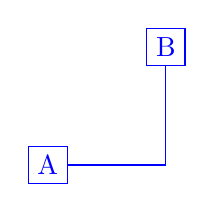
\begin{tikzpicture}[blue]
\node[draw] (A) at (0,0) {A};
\node[draw] (B) at (1.5,1.5) {B};
\draw (A) -| (B);
\end{tikzpicture}
\\ \hline  
(A){\color{red} - -} (B) & (A) {\color{red}|-} (B) &  (A) {\color{red}-|} (B)
\\ \hline 
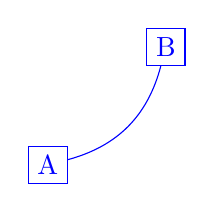
\begin{tikzpicture}[blue]
\node[draw] (A) at (0,0) {A};
\node[draw] (B) at (1.5,1.5) {B};
\draw (A) to [bend right] (B);
\end{tikzpicture}
&  
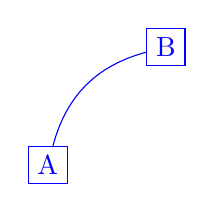
\begin{tikzpicture}[blue]
\node[draw] (A) at (0,0) {A};
\node[draw] (B) at (1.5,1.5) {B};
\draw (A) to [bend left] (B);
\end{tikzpicture}
&  
\begin{tikzpicture}[blue]
\node[draw] (A) at (0,0) {A};
\node[draw] (B) at (1.5,1.5) {B};
\draw (A) to[bend left=0] (B);
\end{tikzpicture}
\\ \hline  
(A) to [\RDD{bend right}] (B) & (A) to [\RDD{bend left}] (B) &  (A) to[\RDD{bend left}=0] (B)
\\ \hline 
\begin{tikzpicture}[blue]
\node[draw] (A) at (0,0) {A};
\node[draw] (B) at (1.5,1.5) {B};
\draw (A) to[bend left=120]  (B);
\end{tikzpicture}
&  
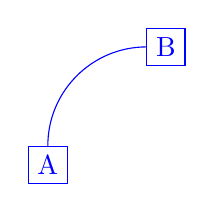
\begin{tikzpicture}[blue]
\node[draw] (A) at (0,0) {A};
\node[draw] (B) at (1.5,1.5) {B};
\draw (A) to[bend left=45] (B);
\end{tikzpicture}
&  
\begin{tikzpicture}[blue]
\node[draw] (A) at (0,0) {A};
\node[draw] (B) at (1.5,1.5) {B};
\draw (A) to[bend left=90] (B);
\end{tikzpicture}
\\ \hline  
(A)  to[\RDD{bend left}=120]  (B) & (A) to[\RDD{bend left}=45] (B) &  (A) to[\RDD{bend left}=90] (B)
\\ \hline 
\begin{tikzpicture}[blue]
\node[draw] (A) at (0,0) {A};
\node[draw] (B) at (1.5,1.5) {B};
\draw (A)  to[out=90]  (B);
\end{tikzpicture}
&  
\begin{tikzpicture}[blue]
\node[draw] (A) at (0,0) {A};
\node[draw] (B) at (1.5,1.5) {B};
\draw (A) to[out=30] (B);
\end{tikzpicture}
&  
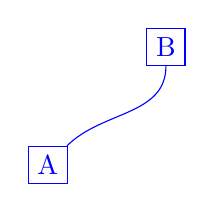
\begin{tikzpicture}[blue]
\node[draw] (A) at (0,0) {A};
\node[draw] (B) at (1.5,1.5) {B};
\draw (A)  to[in=-90]  (B);
\end{tikzpicture}
\\ \hline  
(A)  to[\RDD{out}=90] (B) & (A) to[\RDD{out}=30]  (B) &  (A)  to[\RDD{in}=-90]  (B)
\\ \hline 
%\begin{tikzpicture}[blue]
%\node[draw] (A) at (0,0) {A};
%\node[draw] (B) at (2,2) {B};
%\draw (A)  to[in=90]  (B);
%\end{tikzpicture}
%&  
%\begin{tikzpicture}[blue]
%\node[draw] (A) at (0,0) {A};
%\node[draw] (B) at (2,2) {B};
%\draw (B) to[in=0,out=90]  (B);
%\end{tikzpicture}
%&  
%\begin{tikzpicture}[blue]
%\node[draw] (A) at (0,0) {A};
%\node[draw] (B) at (2,2) {B};
%%\draw (A)  to[out=45,in=-90]  (A);
%\draw (B) to[out=45,in=135] (B);
%\end{tikzpicture}
%\\ \hline  
%(A)  to[\RDD{in}=90] (B) & (B) to[bend left]  (B) & (B) to[out=45,in=135] (B)
%\\ \hline 
\end{tabular} 

\bigskip
\begin{tabular}{|c|c|c|} \hline  
\multicolumn{2}{|c|}{ \BS{draw} (A) .. controls +(right:2cm) and +(down:2cm) .. (B);  }\\ 
\hline  
\begin{tikzpicture}[blue]
\node[draw] (A) at (0,0) {A};
\node[draw] (B) at (2,2) {B};
\draw  (A) .. controls +(right:2cm) and +(down:2cm) .. (B);
\end{tikzpicture}
&
\begin{tikzpicture}[blue]
\node[draw] (A) at (0,0) {A};
\node[draw] (B) at (2,2) {B};
\draw  (A) .. controls +(up:1cm) and +(left:1cm) .. (B);
\end{tikzpicture}
\\ \hline 
controls +(right:2cm) and +(down:2cm)  &
controls +(up:1cm) and +(left:1cm)
\\ \hline 
\begin{tikzpicture}[blue]
\node[draw] (A) at (0,0) {A};
\node[draw] (B) at (2,2) {B};
\draw  (A) .. controls +(right:1cm) and +(right:2cm) .. (B);
\end{tikzpicture}
&
\begin{tikzpicture}[blue]
\node[draw] (A) at (0,0) {A};
\node[draw] (B) at (2,2) {B};
\draw  (A) .. controls +(up:1cm) and +(right:2cm) .. (B);
\end{tikzpicture}
\\ \hline 
controls +(right:1cm) and +(right:2cm)  &
controls +(up:1cm) and +(right:2cm) 
\\ \hline 
\begin{tikzpicture}[blue]
\node[draw] (A) at (0,0) {A};
\node[draw] (B) at (2,2) {B};
\draw  (A) .. controls +(120:2cm) and +(200:1cm) .. (B);
\end{tikzpicture}
 &
 \begin{tikzpicture}[blue]
 \node[draw] (A) at (0,0) {A};
 \node[draw] (B) at (2,2) {B};T
 \draw  (A) .. controls +(120:2cm) and +(200:1cm) .. (A);
 \end{tikzpicture}
\\  \hline  
controls +(120:2cm) and +(200:1cm) & controls +(120:2cm) and +(200:1cm) 
\\ \hline 
\begin{tikzpicture}[blue]
\node[draw] (A) at (0,0) {A};
\node[draw] (B) at (2,2) {B};
\node[draw] (C) at (0,1) {C};
\node[draw] (D) at (3,0) {D};
\draw  (A) .. controls +(C) and +(D) .. (B);
\end{tikzpicture}
&
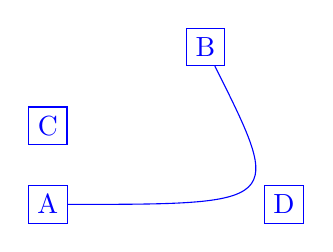
\begin{tikzpicture}[blue]
\node[draw] (A) at (0,0) {A};
\node[draw] (B) at (2,2) {B};
\node[draw] (C) at (0,1) {C};
\node[draw] (D) at (3,0) {D};
\draw (A) .. controls +(D)  .. (B);
\end{tikzpicture}
\\ \hline 
controls +(C) and +(D) &
controls +(D) 
\\ \hline 
\end{tabular} 
 \bigskip
 
\begin{tabular}{|c|c|c|} \hline 
\multicolumn{3}{|l|}{ \BS{node}[draw] (A) at (0,0) \AC{A}  }\\

\multicolumn{3}{|l|}{ \BS{node}[draw] (B) at (2,2) \AC{B} \RDD{edge}  [->] (A);  }\\
\multicolumn{3}{|c|}{\RRR{17-12-1}}  \\
\hline 
 \begin{tikzpicture}
 \node[draw] (A) at (0,0) {A};
 \node[draw] (B) at (2,2) {B} edge [->] (A);
 \end{tikzpicture}
 &
 \begin{tikzpicture}
 \node[draw] (A) at (0,0) {A};
 \node[draw] (B) at (2,2) {B} edge [red]  (A);
 \end{tikzpicture}
 &
 \begin{tikzpicture}
 \node[draw] (A) at (0,0) {A};
 \node[draw] (B) at (2,2) {B} edge [dashed] (A);
 \end{tikzpicture}
\\ \hline 
[->] & [red]  & [dashed]
\\ \hline 
\end{tabular}

%---------------------------------------------------------------------------------
%\subsection{\'Etiquettes sur les n\oe uds}
\SbSSCT{\'Etiquettes sur les n\oe uds}{Node labels}

\begin{tabular}{|c|c|c|c|} \hline
\multicolumn{4}{|c|}{  \BS{fill}(0,0) circle (2pt) node[\RDD{above}] \AC{texte} ;   }\\ 
\hline 
  
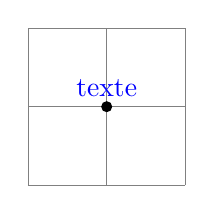
\begin{tikzpicture} \draw[help lines] (-1,-1) grid (1,1) ;\fill (0,0) circle (2pt) node[above] {texte};\end{tikzpicture}
& 
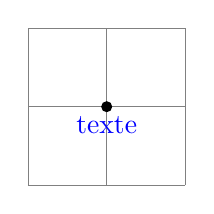
\begin{tikzpicture} \draw[help lines] (-1,-1) grid (1,1) ;\fill (0,0) circle (2pt) node[below] {texte};\end{tikzpicture}
 &  
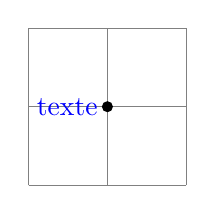
\begin{tikzpicture} \draw[help lines] (-1,-1) grid (1,1);\fill (0,0) circle (2pt) node[left] {texte};\end{tikzpicture}
 &  
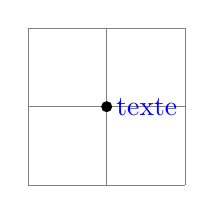
\begin{tikzpicture} \draw[help lines] (-1,-1) grid (1,1); \fill (0,0) circle (2pt) node[right] {texte};\end{tikzpicture}
 \\  \hline 
 [\RDD{above}] & [\RDD{below}] & [\RDD{left}] &  [\RDD{right}]
 \\ \hline 
 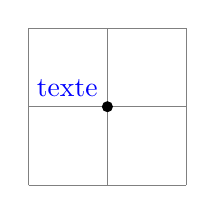
\begin{tikzpicture} \draw[help lines] (-1,-1) grid (1,1) ;\fill (0,0) circle (2pt) node[above left] {texte};\end{tikzpicture}
 & 
 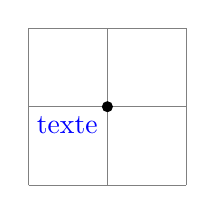
\begin{tikzpicture} \draw[help lines] (-1,-1) grid (1,1) ;\fill (0,0) circle (2pt) node[below left] {texte};\end{tikzpicture}
  &  
 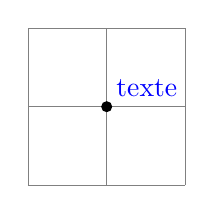
\begin{tikzpicture} \draw[help lines] (-1,-1) grid (1,1);\fill (0,0) circle (2pt) node[above right] {texte};\end{tikzpicture}
  &  
 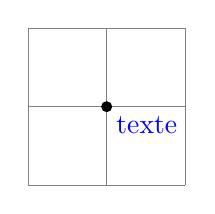
\begin{tikzpicture} \draw[help lines] (-1,-1) grid (1,1); \fill (0,0) circle (2pt) node[below right] {texte};\end{tikzpicture}
  \\  \hline 
  [\RDD{above left}] & [\RDD{below left}] & [\RDD{above right}] &  [\RDD{below right}]
  \\ \hline 
 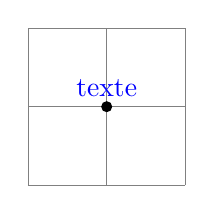
\begin{tikzpicture} \draw[help lines] (-1,-1) grid (1,1) ;\fill (0,0) circle (2pt) node[anchor=south] {texte};\end{tikzpicture}
 & 
 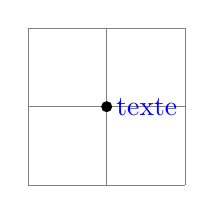
\begin{tikzpicture} \draw[help lines] (-1,-1) grid (1,1) ;\fill (0,0) circle (2pt) node[anchor=west] {texte};\end{tikzpicture}
  &  
 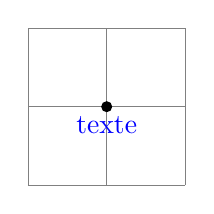
\begin{tikzpicture} \draw[help lines] (-1,-1) grid (1,1);\fill (0,0) circle (2pt) node[anchor=north] {texte};\end{tikzpicture}
  &  
 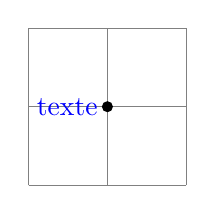
\begin{tikzpicture} \draw[help lines] (-1,-1) grid (1,1); \fill (0,0) circle (2pt) node[anchor=east] {texte};\end{tikzpicture}
  \\  \hline 
  [\RDD{anchor=south}] & [\RDD{anchor=west}] & [\RDD{anchor=north}] & [\RDD{anchor=east                                                                                                                                                               }]
  \\ \hline 
 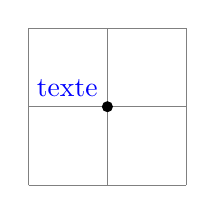
\begin{tikzpicture} \draw[help lines] (-1,-1) grid (1,1) ;\fill (0,0) circle (2pt) node[anchor=south east] {texte};\end{tikzpicture}
 & 
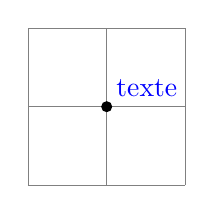
\begin{tikzpicture} \draw[help lines] (-1,-1) grid (1,1) ;\fill (0,0) circle (2pt) node[anchor=south west] {texte};\end{tikzpicture}
&  
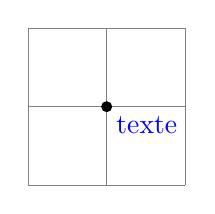
\begin{tikzpicture} \draw[help lines] (-1,-1) grid (1,1);\fill (0,0) circle (2pt) node[anchor=north west] {texte};\end{tikzpicture}
&  
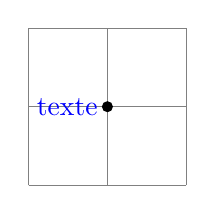
\begin{tikzpicture} \draw[help lines] (-1,-1) grid (1,1); \fill (0,0) circle (2pt) node[anchor=east] {texte};\end{tikzpicture}
\\  \hline 
[\RDD{anchor=south east}] & [\RDD{anchor=south west}] & [\RDD{anchor=north west}] & [\RDD{anchor=north east                                                                                                                                                              }]
  \\ \hline 
\end{tabular} 


\bigskip
\begin{tabular}{|c|c|c|c|} \hline
\multicolumn{4}{|c|}{  \BS{fill}(0,0) circle (2pt) node[\RDD{above}=.3cm] \AC{texte} ;   }\\ 
\hline 
  
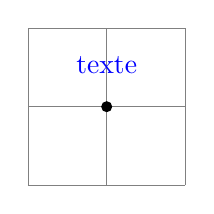
\begin{tikzpicture} \draw[help lines] (-1,-1) grid (1,1) ;\fill (0,0) circle (2pt) node[above=.3cm] {texte};\end{tikzpicture}
& 
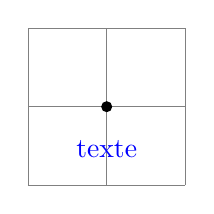
\begin{tikzpicture} \draw[help lines] (-1,-1) grid (1,1) ;\fill (0,0) circle (2pt) node[below=.3cm] {texte};\end{tikzpicture}
 &  
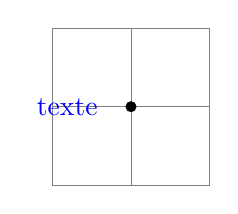
\begin{tikzpicture} \draw[help lines] (-1,-1) grid (1,1);\fill (0,0) circle (2pt) node[left=.3cm] {texte};\end{tikzpicture}
 &  
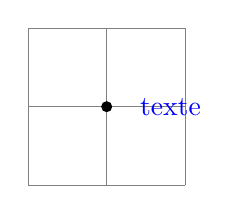
\begin{tikzpicture} \draw[help lines] (-1,-1) grid (1,1); \fill (0,0) circle (2pt) node[right=.3cm] {texte};\end{tikzpicture}
 \\  \hline 
 [\RDD{above}=.3cm] & [\RDD{below}=.3cm] & [\RDD{left}=.3cm] &  [\RDD{right}=.3cm]]
 \\ \hline 
\begin{tikzpicture} \draw[help lines] (-1,-1) grid (1,1) ;\fill (0,0) circle (2pt) node[above left=.3cm] {texte};\end{tikzpicture}
& 
\begin{tikzpicture} \draw[help lines] (-1,-1) grid (1,1) ;\fill (0,0) circle (2pt) node[below left=.3cm] {texte};\end{tikzpicture}
 &  
\begin{tikzpicture} \draw[help lines] (-1,-1) grid (1,1);\fill (0,0) circle (2pt) node[above right=.3cm] {texte};\end{tikzpicture}
 &  
\begin{tikzpicture} \draw[help lines] (-1,-1) grid (1,1); \fill (0,0) circle (2pt) node[below right=.3cm] {texte};\end{tikzpicture}
 \\  \hline 
 [\RDD{above left}=.3cm] & [\RDD{below left}=.3cm] & [\RDD{above right}=.3cm] &  [\RDD{below right}=.3cm]]
 \\ \hline 
 
 \end{tabular} 
 
%\begin{tikzpicture} \draw[help lines] (-1,-1) grid (1,1);\fill (0,0) circle (2pt) node[distance=.3cm] {texte};\end{tikzpicture} 
 
 \newpage
\selectlanguage{french}
 
 \begin{tabular}{|c|c|c|c|c|} \hline
 \multicolumn{5}{|l|}{ \BSS{shorthandoff}\AC{:} \footnotemark[1]  } \\
 \multicolumn{5}{|l|}{  \BS{node} [draw,\RDD{label}=right:texte] \AC{}   }\\
 \multicolumn{5}{|l|}{ \BSS{shorthandon}\AC{:} } \\ 
 \hline 
     \shorthandoff{:} 
 \tikz \node [draw,label=right:texte] {};
 \shorthandon{:}
 &
  \shorthandoff{:}
 \tikz \node [draw,label=left:texte] {};
 \shorthandon{:}
 &
  \shorthandoff{:}
 \tikz \node [draw,label=above:texte] {};
 \shorthandon{:}
 &
  \shorthandoff{:}
 \tikz \node [draw,label=below:texte] {};
 \shorthandon{:}
 &
  \shorthandoff{:}
 \tikz \node [draw,label=45:texte] {};
    \shorthandon{:}
   \\ \hline
  label=right & label=left &  label=above & label=below & label=45
    \\ \hline 
 \end{tabular}
 \footnotetext[1]{\TFRGB{désactivation et ré-activation de \og : \fg  conflit entre les modules Tikz et Babel en français}{Only useful when the package babel is loaded with the frenchb option    }}
 
 \bigskip
  \begin{tabular}{|c|c|c|c|c|} \hline
  \BS{fill}(0,0) circle (2pt) node[below right=.3cm,draw,label=45:étiquette] \AC{texte} ;
      \\ \hline 
  
  \shorthandoff{:}
\begin{tikzpicture} \draw[help lines] (-1,-1) grid (2,1); \fill (0,0) circle (2pt) node[below right=.3cm,draw,label=45:étiquette] {texte};\end{tikzpicture}
 \shorthandon{:}
 
    \\ \hline 
 \end{tabular}
\bigskip

 \shorthandoff{:}
 

 
\begin{tabular}{|c|c|c|} \hline
\multicolumn{3}{|c|}{  \BSS{shorthandoff}\AC{:} \BS{node}[circle,draw,blue,\RDD{pin}=texte] \AC{} ;   \BSS{shorthandon}\AC{:}  \footnotemark[1] }\\ 
\hline
\begin{tikzpicture} 
\node [circle,draw,blue,pin=texte] {};
\end{tikzpicture}
&
\begin{tikzpicture} 
\node [circle,draw,blue,pin=60:texte] {};
\end{tikzpicture}
&
\begin{tikzpicture} 
\node [circle,draw,blue,pin=right:texte] {};
\end{tikzpicture}
 \\ \hline
[circle,pin=texte] &   [circle,pin=60:texte] & [circle,pin=right:texte]
 \\ \hline 
\end{tabular}  

\bigskip
\begin{tabular}{|c|c|c|} \hline
\multicolumn{3}{|c|}{  \BS{tikz}[\RDD{pin position}=60] \BS{node} [circle,pin=texte] \AC{} ;   }\\ 
\hline 
\tikz[pin position=60] \node [circle,draw,blue,pin=texte] {};
&
\tikz[pin distance=0 cm] \node [circle,draw,blue,pin=60:texte] {};
&
\tikz[pin distance=2 cm] \node [circle,draw,blue,pin=60:texte,pin distance=0cm] {};
  \\ \hline
  [\RDD{pin position}=60] & [\RDD{pin distance}=0 cm] & [\RDD{pin distance}=2 cm]
    \\ \hline
  \dft{ : above} & \multicolumn{2}{|c|}{ \dft{ : 3 ex}}
      \\ \hline
\end{tabular}  

% % % % % % % % % % >>>>>>>>>> a voir : option edge <<<<<<<<<<<<<<<<<<<<<<<<<<<<<<<<<<<<<<

   \shorthandon{:} 
   
\selectlanguage{english}   
% >>>>>>>>>>>>>>>>>>>>>> A Voir : positioning librairy <<<<<<<<<<<<<<<<<<<<<<<<<<<<<<<<<<<<<<<

%\subsection{ N\oe uds  sur un chemin}
\SbSSCT{ N\oe uds  sur un chemin}{Nodes on a path}

\begin{tabular}{|c|c|c|} \hline
\multicolumn{3}{|c|}{  \BS{draw}(0,0) .. controls (1,2) and (2,-1) .. (4,0) node[\RDD{at end}] \AC{texte} ;   }\\ 
\hline 
\tikz \draw (0,0) .. controls (1,2) and (2,-1) .. (4,0) node[pos=0] {texte}; 
&
\tikz \draw (0,0) .. controls (1,2) and (2,-1) .. (4,0) node[pos=.33] {texte}; 
&
\tikz \draw (0,0) .. controls (1,2) and (2,-1) .. (4,0) node[at end] {texte}; 
  \\ \hline 
\RDD{pos}{\color{red}  =0} & \RDD{pos}{\color{red}  =.33} & \RDD{at end} (pos=1)
  \\ \hline 

\tikz \draw (0,0) .. controls (1,2) and (2,-1) .. (4,0) node[very near end] {texte}; 
&
\tikz \draw (0,0) .. controls (1,2) and (2,-1) .. (4,0) node[near end] {texte}; 
&
\tikz \draw (0,0) .. controls (1,2) and (2,-1) .. (4,0) node[midway] {texte}; 
  \\ \hline 
\RDD{very near end} (pos=0.875.) & \RDD{ near end} (pos=0.75) & \RDD{midway} (pos=0.5)
  \\ \hline 
  
\tikz \draw (0,0) .. controls (1,2) and (2,-1) .. (4,0) node[near start] {texte}; 
&
\tikz \draw (0,0) .. controls (1,2) and (2,-1) .. (4,0) node[very near start] {texte}; 
&
\tikz \draw (0,0) .. controls (1,2) and (2,-1) .. (4,0) node[at start] {texte};
\\ \hline 
\RDD{near start} (pos=0.25) & \RDD{very near start} (pos=0.125) & \RDD{at start} (pos=0)
  \\ \hline 
  
\end{tabular} 

\bigskip
\begin{tabular}{|c|c|c|} \hline
\multicolumn{3}{|c|}{  \BS{draw}(0,0) .. controls (1,2) and (2,1) .. (4,0) node[\RDD{sloped},midway] \AC{texte} ;   }\\ 
\hline 
\tikz \draw (0,0) .. controls (1,2) and (2,-1) .. (4,0) node[sloped,midway] {texte};
&
\tikz \draw (0,0) .. controls (1,2) and (2,-1) .. (4,0) node[above,midway] {texte};
&
\tikz \draw (0,0) .. controls (1,2) and (2,-1) .. (4,0) node[below,midway] {texte};
  \\ \hline
\RDD{sloped} & \RDD{above} &\RDD{below}
  \\ \hline
\end{tabular}
\bigskip

\begin{tabular}{|c|c|c|} \hline
\multicolumn{3}{|c|}{  \BS{draw}(0,0) .. controls (1,2) and (2,1) .. (5,0) node[\RDD{sloped},midway,allow upside down] \AC{texte} ;   }\\ 
\hline 
\tikz \draw (0,0) .. controls (1,2) and (2,-1) .. (4,0) node[sloped,midway,allow upside down] {texte};
&
\tikz \draw (0,0) .. controls (1,2) and (2,-1) .. (4,0) node[above,midway,allow upside down] {texte};
&
\tikz \draw (0,0) .. controls (1,2) and (2,-1) .. (4,0) node[below,midway,allow upside down] {texte};
  \\ \hline
\RDD{sloped} & \RDD{above} &\RDD{below}
  \\ \hline
\end{tabular}  


\begin{tabular}{|c|c|c|} \hline
\multicolumn{3}{|c|}{  \BS{draw}(A)  to [bend right]  node [\RDD{bend right}] \AC{texte} (B);   }\\ 
\hline 
\begin{tikzpicture} %[auto,bend right]
\node[draw] (A) at (0,0) {A};
\node[draw] (B) at (2,2) {B};
\draw (A) to [bend right] node [bend right] {texte} (B);
\end{tikzpicture}
&
\begin{tikzpicture} 
\node[draw] (A) at (0,0) {A};
\node[draw] (B) at (2,2) {B};
\draw (A) to [bend right] node [auto,bend right] {texte} (B);
\end{tikzpicture}
&
\begin{tikzpicture} 
\node[draw] (A) at (0,0) {A};
\node[draw] (B) at (2,2) {B};
\draw (A) to[bend right] node [auto,swap,bend right] {texte} (B);
\end{tikzpicture}
  \\ \hline
[bend right]  & [\RDD{auto},bend right] & [auto,\RDD{swap},bend right] 
  \\ \hline
\end{tabular}  

\SbSSCT{ N\oe uds  sur un \og edge\fg}{Nodes on an edge}

\begin{tabular}{|c|c|c|}\hline  
\multicolumn{3}{|c|}{  \BS{draw}(0,0) edge \BDD{["abc", ->]} (4,0);  }\\ 
\multicolumn{3}{|c|}{  \RRR{17-12-2} }\\ 
\hline 
\begin{tikzpicture}[blue] 
\useasboundingbox  (0,-.5) rectangle (4,.5); 
\draw (0,0) edge ["abc", ->] (4,0);
\end{tikzpicture}
&
\begin{tikzpicture}[blue] 
\useasboundingbox  (0,-.5) rectangle (4,.5); 
\draw (0,0) edge ["abc", near start] (4,0);
\end{tikzpicture}
&
\begin{tikzpicture}[blue] 
\useasboundingbox  (0,-.5) rectangle (4,.5); 
\draw (0,0) edge ["abc", style={auto=right}] (4,0);
\end{tikzpicture}
\\ \hline 
["abc", ->]
& 
["abc", near start] &  ["abc", style=\AC{auto=right}] 
\\ \hline  
\begin{tikzpicture}[blue] 
\useasboundingbox  (0,-.5) rectangle (4,.5); 
\draw (0,0) edge [font=\Large,"abc" ] (4,0);
\end{tikzpicture}
&
\begin{tikzpicture}[blue] 
\useasboundingbox  (0,-.5) rectangle (4,.5); 
\draw (0,0) edge ["abc" color=red ] (4,0);
\end{tikzpicture}
&
\begin{tikzpicture}[blue] 
\useasboundingbox  (0,-.5) rectangle (4,.5); 
 \draw (0,0) edge ["abc" '] (4,0);
\end{tikzpicture}
\\ \hline 
[font=\BS{Large},"abc" ] & ["abc" color=red ]
&["abc" ' ]
\\ \hline 

\begin{tikzpicture}[blue] 
\useasboundingbox  (0,-.5) rectangle (4,.75); 
\draw (0,0) edge ["abc" draw ] (4,0);
\end{tikzpicture}
&
\begin{tikzpicture}[blue] 
\useasboundingbox  (0,-.5) rectangle (4,.5); 
\draw (0,0) edge ["abc" inner sep=0pt ] (4,0);
\end{tikzpicture}
&
\begin{tikzpicture}[blue] 
\useasboundingbox  (0,-.5) rectangle (4,.5); 
\draw (0,0) edge ["abc" fill ,fill=yellow ] (4,0);
\end{tikzpicture}
\\ \hline
["abc" draw ]
&
["abc" inner sep=0pt ]
&
["abc" fill ,fill=yellow ]
\\ \hline
\end{tabular} 



\bigskip

\begin{tabular}{|c|} \hline  
\BS{draw}[every edge quotes/.style=\AC{fill=yellow}] (0,0) edge ["abc"] (4,0);
\\ \hline  
\begin{tikzpicture}[blue] 
\useasboundingbox  (0,-.5) rectangle (4,.5); 
 \draw[every edge quotes/.style={fill=yellow}] (0,0) edge ["abc"] (4,0);
\end{tikzpicture}
\\ \hline 
\end{tabular} 




